\documentclass[10pt,pdf,hyperref={unicode}]{beamer}

\let\Tiny=\tiny
\usepackage[T2A]{fontenc}
\usepackage[utf8x]{inputenc}
\usepackage{ucs}
\usepackage[english,russian]{babel}
\usepackage{lmodern}
\usepackage{graphicx}

\renewcommand{\rmdefault}{cmr} % Шрифт с засечками
\renewcommand{\sfdefault}{cmss} % Шрифт без засечек
\renewcommand{\ttdefault}{cmtt} % Моноширинный шрифт

\begin{document}

\title[VBR Modelling]
{Обзор подходов к моделированию VBR потоков}
\date{\today}

\frame{\titlepage}

\begin{frame}
    \frametitle{Введение}
    При проектировании сети необходимо учитывать характер
    входной нагрузки. Тестировать сеть на реальных видео
    слишком затратно, а к достаточно полным (и объёмным)
    базам трейсов доступ может быть ограничен.\\[0.5 cm]

    Одним из решений этой проблемы является моделирование
    входного потока с учётом его статистических свойств
    и анализ сети с помощью модели.\\[0.5 cm]

    A Survey of VBR Video Traffic Models [Tanwir, Perros] (2013)
\end{frame}

\begin{frame}
    \frametitle{Характеристики видеопотока}
    Моделируемым потоком является поток размеров
    кадров на выходе кодера для видеоконференции
    (говорящая голова).
    \begin{itemize}
        \item ``Куполообразное'' распределение размеров кадров
        \item Ярко выраженная автокорреляция, имеющая экспоненциальный
            характер убывания
    \end{itemize}
\end{frame}

\begin{frame}
    \begin{figure}[h]
        \begin{center}
            \includegraphics[width=\textwidth]{akiyo_sizes.png}
        \end{center}
        \caption{Размеры кадров от времени (Akiyo)}
        \label{fig:akiyo_sizes}
    \end{figure}
\end{frame}

\begin{frame}
    \begin{figure}[h]
        \begin{center}
            \includegraphics[width=\textwidth]{akiyo_hist.png}
        \end{center}
        \caption{Гистограмма размеров кадров (Akiyo)}
        \label{fig:akiyo_hist}
    \end{figure}
\end{frame}

\begin{frame}
    \begin{figure}[h]
        \begin{center}
            \includegraphics[width=\textwidth]{miss-america.png}
        \end{center}
        \caption{Гистограмма размеров кадров (Miss America)}
        \label{fig:miss_america_hist}
    \end{figure}
\end{frame}

\begin{frame}
    \begin{figure}[h]
        \begin{center}
            \includegraphics[width=\textwidth]{akiyo_acf.png}
        \end{center}
        \caption{Автокорреляционная функция, zoom-in (Akiyo)}
        \label{fig:akiyo_acf}
    \end{figure}
\end{frame}

\begin{frame}
    \begin{figure}[h]
        \begin{center}
            \includegraphics[width=\textwidth]{akiyo_acf_long.png}
        \end{center}
        \caption{Автокорреляционная функция, zoom-out (Akiyo)}
        \label{fig:akiyo_acf_long}
    \end{figure}
\end{frame}

\begin{frame}
    \frametitle{Критерии выбора (и создания) моделей}
    \begin{itemize}
        \item Различные типы кадров: Да
        \item Автокорреляционные характеристики: Да
        \item Short-Range Dependencies (SRD): Да
        \item Long-Range Dependencies (LRD): Нет
        \item Смена сцены: Нет
        \item Interleaved (Multiple) sources:~?
        \item ``Универсальность'' vs Количество параметров:~?
        \item ``Хвост'' распределения:~?
    \end{itemize}
\end{frame}

\begin{frame}
    \frametitle{Классификация моделей}
    \begin{itemize}
        \item Авторегрессионные модели
        \item Марковские модели
        \item Самоподобные (self-similar) и ARIMA
        \item Вейвлетные модели
        \item Прочие (M/G/$\infty$, TES etc)
    \end{itemize}
\end{frame}

\begin{frame}
    \frametitle{Авторегрессионные модели}
    \begin{itemize}
        \item AR. Взвешенная сумма + ``остаточный процесс'' (residual process)
        $$
            x(n) = \sum_{i=1}^{p}{a_i x(n - i)} + e(n)
        $$
        \item DAR(p). Нужное распределение вероятностей ($Y_n$) и автокорреляционная
            функция ($A_n$). Считается, что DAR(1) подходит только для множественных
            каналов (multiple source). Почему?
        $$
            X_n = V_nX_{n - A_n} + (1 - V_n) Y_n
        $$
        \item Frame-Based AR. Надстройка над AR для учёта смены сцен.
    \end{itemize}

    Авторегрессионные процессы отлично описывают трафик видеоконференции,
    но плохо подходят для full motion. Можно подбирать ``базовое'' распределение,
    подстраиваясь под специфику моделируемого потока (Normal, Lognormal, Gamma,
    Pearson V, Negative binomial, Gamma/Pareto etc).
\end{frame}

\begin{frame}
    \begin{figure}[h]
        \begin{center}
            \includegraphics[width=\textwidth]{miss-america-hist-dar.png}
        \end{center}
        \caption{DAR(1) vs Trace, гистограмма (MA)}
        \label{fig:hist_cmp_miss}
    \end{figure}
\end{frame}

\begin{frame}
    \begin{figure}[h]
        \begin{center}
            \includegraphics[width=\textwidth]{acf_cmp_miss.png}
        \end{center}
        \caption{DAR(1) vs Trace, aвтокорреляционная функция (MA)}
        \label{fig:acf_cmp_miss}
    \end{figure}
\end{frame}

\begin{frame}
    \frametitle{Марковские модели}
    Текущее состояние ``доминирующего процесса'' зависит
    только от предыдущего состояния. Марковский процесс
    часто контролирует параметры некоторого другого процесса,
    например, авторегрессионного.
    \begin{itemize}
        \item State = GOP Size
        \item State = Scene class
        \item State = Frame size (a lot of states)
    \end{itemize}
    Конкретные примеры:
    \begin{itemize}
        \item Markov Renewal Process Model (MRP) (equidistant)
        \item Markov-Modulated AR Models (scene changes)
        \item Markov-Modulated Gamma Model (scene changes)
    \end{itemize}

    Большая часть марковских моделей была создана для учёта
    смены сцен в видеопоследовательностях. Подбор параметров
    является сложной задачей (иногда подбор границ активности
    сцен осуществляется вручную!). Алгоритм Макса-Ллойда для MRP?
\end{frame}

\begin{frame}
    \frametitle{Самоподобные (self-similar) модели}
    LRD (Long-Range Dependent) процесс является самоподобным,
    если для любых значений смещения и после усреднения по
    блокам любой длины $m$ коэффициент автокорреляции остаётся
    неизменным.\\[0.5 cm]

    Long-Range Dependence (зависимость с большой памятью - авт.) ---
    явление, при котором текущие значения случайного процесса
    сильно коррелированы со значениями, удалёнными во времени.\\[0.5 cm]

    Степень зависимости во времени характеризуется параметром
    Хёрста $0.5 < H < 1$. Этот параметр оценивается по трейсу и
    подаётся на вход самоподобному случайному процессу.\\[0.5 cm]

    Самоподобные модели разрабатывались для full motion.
    Неспособны точно отражать SRD. Характеризуются
    степенной ACF. Для трафика видеоконференций типичное
    значение параметра Хёрста -- $0.6$.
\end{frame}

\begin{frame}
    \frametitle{Вейвлетные модели}
    \begin{itemize}
        \item Применяем вейвлетное преобразование к трейсу
        \item Оцениваем корреляцию коэффициентов вейвлетного преобразования
        \item Генерируем новые коэффициенты WT на основе построенной модели
        \item Применяем обратное вейвлетное преобразование, получаем
            синтезированный трейс.
    \end{itemize}
    В чём особенности и преимущества вейвлетных моделей:
    \begin{itemize}
        \item Не требуется дополнительной надстройки для учёта смены сцен
        \item Точно отражает как близкие, так и дальние зависимости
        \item Дальние зависимости по времени переходят в близкие
            зависимости коэффициентов преобразования.
    \end{itemize}

    Трафик видеоконференций не LRD (подтвердить). Вейвлетные модели
    представляются избыточными.
\end{frame}

\begin{frame}
    \frametitle{M/G/$\infty$}
    \begin{itemize}
        \item ACF for LRD: $\rho (k) = k^{-\beta} = e^{-\beta \log k}$
        \item ACF for Markov: $\rho(k) = e^{-\beta k}$
        \item Best fit ACF: $\rho(k) = e^{-\beta \sqrt{k}}$\\[0.5 cm]
    \end{itemize}

    Для процесса M/G/$infty$ авторы аналитически вывели pmf для
    G так, чтобы количество занятых серверов обладало требуемыми
    автокорреляционными характеристиками. Далее производится
    преобразование полученной случайной величины таким образом,
    чтобы свести распределение вероятностей к целевому (Gamma/Pareto).\\[0.5 cm]

    ACF для видеоконференций хорошо моделируется экспоненциальным законом
    (AR/Markovian подходят), необходимость в данной модели под вопросом.
\end{frame}

\begin{frame}
    \frametitle{Методы сравнения моделей}
    \begin{itemize}
        \item Статистические критерии
        \begin{itemize}
            \item Q-Q plot
            \item первые два момента
            \item ACF
        \end{itemize}

        \item QoS network metrics (!)
        \begin{itemize}
            \item Loss Rate
            \item Delay
            \item Jitter
        \end{itemize}
    \end{itemize}

    Статистические критерии дают немного информации о
    порядке следования кадров (SRD?). Схожесть модели
    и исходного трейса оценивают по их поведению при
    симуляции передачи по сети.
\end{frame}

\begin{frame}
    \begin{figure}[h]
        \begin{center}
            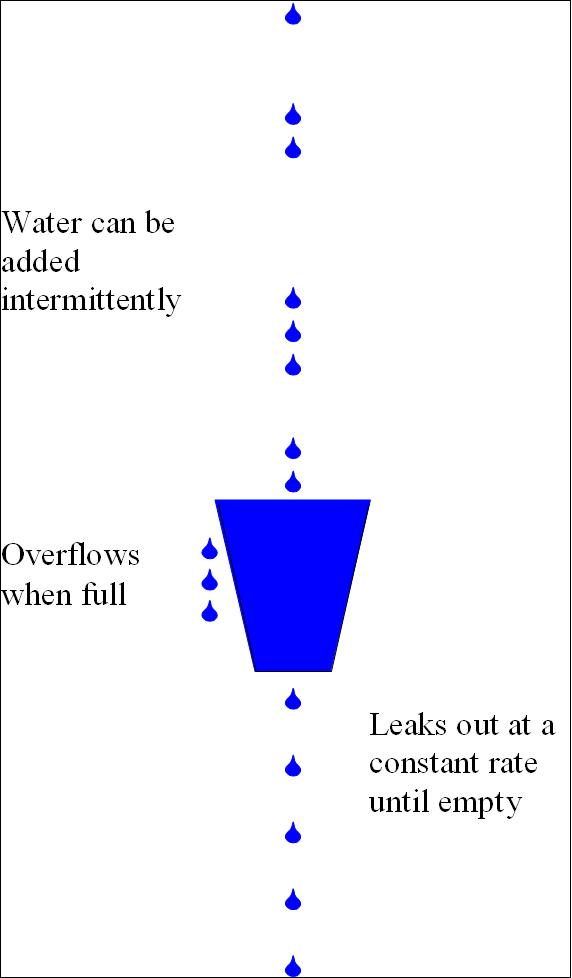
\includegraphics[height=0.8\textheight]{leaky_bucket_analogy.jpg}
        \end{center}
        \caption{Leaky bucket, literally}
        \label{fig:leaky_bucket}
    \end{figure}
\end{frame}

\begin{frame}
    \frametitle{Выводы, TODO}
    \begin{itemize}
        \item Большая часть моделей ``мимо кассы''.
        \item Проверить LRD
        \item Важен ли ``хвост'' основного распределения?
        \item Нормально ли ACF аппроксисмируется экспонентой?
        \item Никто не публиковал сравнения на основе QoS-параметров
            IP-сетей (в обзорной статье это записано в FW).
        \item Оптимальное квантование для MRP - хорошая идея?
        \item Почему DAR не подходит для single-source?
        \item Нигде не использовался DAR(p) + Gamma/Pareto
    \end{itemize}
\end{frame}

\end{document}
